\section{Lattice and Algorithm} \label{sec:cmpalgo}

The \cmp (CMP) model is a cellular automaton which shows fibrillation-like behaviour. The myocardium is represented by a square lattice with side length $L$, and discrete sites, each representing a single cardiomyocyte. Sites can be coupled to their nearest neighbours, which means that they can interact; these couplings are analogous to the gap junctions in cardiomyocytes. Each site is coupled to its neighbours in the `longitudinal' direction (left-right in Fig.~\ref{fig:cmp}) 100\% of the time, whereas it is coupled to its neighbours in the `transverse' direction (up-down in Fig.~\ref{fig:cmp}) with some probability $\nu$. This reflects the structure of the myocardium, in which cells are arranged in long fibres which occasionally branch to form transverse connections~\cite{de2011fibrosis}. In the transverse direction, there are periodic boundary conditions, meaning that this lattice is really a thin cylindrical shell. This very loosely approximates the topology of a real atrium~\cite{cmp}.

 \begin{figure}[b!] \begin{mdframed}
 	\centering
 	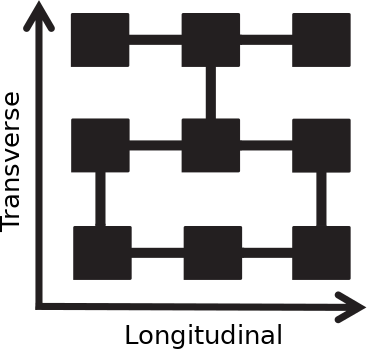
\includegraphics[width=0.45\linewidth]{cmp}
 	\caption{Diagram of an example CMP model lattice with $L=3$. The black boxes represent cardiomyocytes and the couplings between them represent gap junctions between cardiomyocytes. The sites in the leftmost column are the pacemakers, which spontaneously excite at a regular rate. In the left-right direction, every possible nearest-neighbour coupling exists. In the up-down direction, nearest-neighbour couplings exist with probability $\nu$. This reflects the branching structure of the myocardium, which has long fibres with occasional transverse connections between them. The labels `transverse' and `longitudinal' are therefore a natural choice when labelling the two axes. Adapted from~\cite{cmp}.}
 	\label{fig:cmp}
 \end{mdframed} \end{figure}

Each site in the model has three possible states, updated at each timestep of the model based on their own state and that of their coupled neighbours. The allowed states (and their corresponding phases in the cardiac action potential shown in Fig.~\ref{fig:atrialcap}) are:
\begin{itemize}
    \item excited (phase 0)
    \item resting (phase 4)
    \item refractory (phases 1--3).
\end{itemize}
The sites on the leftmost edge of the lattice are defined to be `pacemaker' sites, analogous to the sinoatrial node in the atrium. Their states are set to excited each time a fixed number of timesteps has elapsed.
5\% of sites (chosen randomly) are designated `defective', meaning they have a 5\% chance of failing to excite when the model rules dictate they should~\cite{cmp}.

The rules determining the evolution of the state of each site are shown in flowchart form in Fig.~\ref{fig:cmpalgo}. Based on these simple rules, a propagating signal arises, analogous to the electrical signal that propagates through the atrium~\cite{cmp}.

Re-entry circuits can arise in the model when a defective site fails to excite. Figure~\ref{fig:cmpreentry} explains how a re-entry circuit might form, and why they form more often when $\nu$ is small. Note that this is the simplest example of a re-entry circuit; circuits found in the model can be far more complicated than the example shown and often multiple re-entry circuits may form at the same time.

In order to determine computationally whether the system is fibrillating, we tracked the number of times each site was excited. If the site with the highest number of excitations was a pacemaker, then the system was not fibrillating. Otherwise, we concluded that a site has been excited more times than the pacemakers and therefore must be part of a re-entry circuit. This metric was chosen because it generalises well to 3D and more complicated geometries. More obvious metrics like `number of sites excited at a given time greater than some threshold' only work in this very simple 2D model because it is homogeneous at large scales and so the number of excited cells changes little over a pacemaker period. However, it must be noted that this choice of metric introduces a source of error to the model: re-entry circuits are only detected after they complete their first loop, and their termination is only detected after the subsequent excitation of the pacemakers. When measuring the number of timesteps spent in AF, this introduces an error of up to approximately one pacemaker period per episode of AF. % TODO how negligible?

\begin{figure}
	\centering
    \begin{tikzpicture}[node distance=5cm,align=center,auto]
	\node[decision](start){What is the \\ state of the cell?};
    \node[block, above of=start](realstart){Start};
	\node[decision, below of=start, node distance=4.5cm](refractory){Has cell been \\ refractory for \\ $\tau$ timesteps?};
	\node[decision, right of=start, node distance=5.5cm](excited){Are any excited \\ cells coupled \\ to this one?};
	\node[decision, below of=excited, node distance=4.5cm](pacemaker){Is the cell \\ a pacemaker?};
	\node[decision, below of=pacemaker, node distance=4.5cm](pacemakerperiod){Is the time \\ elapsed a \\ multiple of $T$?};
	\node[decision, right of=pacemaker, node distance=5.5cm](defective){Is the cell \\ defective?};
	\node[decision, below of=defective](defectivecheck){Generate a \\ random \\ uniform \\ $U \in [0, 1]$};
	\node[block, below of=pacemakerperiod, node distance=4cm](excitedend){Excited};
	\node[block, left of=excitedend, node distance=5.5cm](restingend){Resting};
	\node[block, left of=restingend, node distance=3.0cm](refractoryend){Refractory};
	\node[block, right of=excitedend, node distance=5.5cm](restingend2){Resting};
	
	\path[line](realstart)       -- (start);
	\path[line](start)           -- node[very near start]{refractory} (refractory);
	\path[line](refractory)      -| node[very near start]{no}         (refractoryend);
	\path[line](refractory)      -- node[pos=0.05]{yes}        (restingend);
	\path[line](start)           -- node[pos=0.3]{resting}    (excited);
	\path[line](excited)         -- node[very near start]{no}         (pacemaker);
	\path[line](pacemaker)       -- node[very near start]{yes}        (pacemakerperiod);
	\path[line](pacemaker.west) -| node[above, very near start]{no} ++(-0.6, 0) |- (restingend);
	\path[line](excited)         -| node[pos=0.05]{yes}        (defective);
	\path[line](defective)       -- node[very near start]{yes}        (defectivecheck);
	\path[line](defective.west) -| node[above, very near start]{no} ++(-1.05, 0) |-         (excitedend);
	\path[line](defectivecheck)  -- node[very near start]{$U < \epsilon$}         (restingend2);
	\path[line](defectivecheck.west) -| node[above, pos=0.2]{$U \ge \epsilon$} ++(-1.05, 0) |- (excitedend);
	\path[line](pacemakerperiod) -- node[very near start]{yes}        (excitedend);		
	\path[line](pacemakerperiod.west) -| node[above, very near start]{no} ++(-0.6, 0) |- (restingend);
	\path[line](start)           -| node[above, pos=0.3]{excited}    (refractoryend);
	
	\path[line] (defective.west) -- ++(-1.05, 0);
	\path[line] (defectivecheck.west) -- ++(-1.05, 0);
	\path[line] (pacemaker.west) -- ++(-0.6, 0);
	\path[line] (pacemakerperiod.west) -- ++(-0.6, 0);
	\path[line] (refractory.west) -- ++(-1.00, 0);
	\path[line] (start.west) -- ++(-1.00, 0);
\end{tikzpicture}
    \caption{The algorithm used to determine the next state of the cell; this should be run for every cell in the lattice and the results should be stored before making any changes. Then, all state changes can be applied at once. $\tau$ is the refractory period of each heart cell, $T$ is the pacemaker period, and $\epsilon = 0.05$ is the probability of a defective cell failing to excite.}
    \label{fig:cmpalgo}
\end{figure}

\begin{figure} \begin{mdframed}
	\centering
	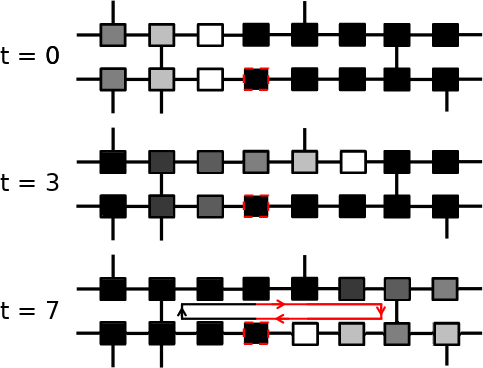
\includegraphics[width=0.7\linewidth]{cmp_reentry_2}
	\caption[short caption]{Diagram showing the formation of a simple re-entry circuit. A white square is an excited cell; a black square is a resting cell. Refractory cells start off light grey and progress to dark grey.
	At $t=0$, a signal is propagating along both the upper and lower branch. The red box indicates a defective cell, which fails to excite at $t=1$ thus extinguishing the signal along the lower branch, which is why at $t=3$ there is only conduction along the upper branch. At $t=7$, it can be seen that the signal has crossed over a transverse connection onto the lower branch. From here it is obvious that the signal can keep propagating in a loop until the defective cell fails again (which only happens with probability 5\%).
	Note that if the right transverse connection was too close to the left one, there would still be refractory cells on the lower branch by the time the wavefront looped back around, and the circuit would be extinguished. This is why there are no circuits for large $\nu$. This also explains why for small $\nu$ the fibrillation is persistent; in this regime, many re-entry circuits form so the chance of all of them being inactive at the same time is vanishingly small. 
	This large gap between transverse fibres is analogous to an anatomical obstacle, so re-entry circuits in the CMP model are anatomical rather than functional. Diagram adapted from~\cite{cmp}.}
	\label{fig:cmpreentry}
\end{mdframed} \end{figure}

\clearpage
\section{Results from Literature}


There is a threshold value of the connection fraction $\nu = \nu^*$. When $\nu \gg \nu^*$, no re-entry circuits form and the wave propagates longitudinally. When $\nu \ll \nu^*$, re-entry circuits form spontaneously and produce persistent fibrillation. When $\nu \approx \nu^*$, self-terminating or `paroxysmal' AF appears. In the real myocardium, the transverse connectivity is reduced by fibrosis, which has been implicated in atrial fibrillation~\cite{de2011fibrosis}. This result is therefore consistent with clinical observations. This dependence of atrial fibrillation risk on $\nu$ is summarised in Fig.~\ref{fig:cmpriskcurve}. It is possible to derive a theoretical form of this `risk curve' by neglecting boundary effects:
\begin{equation}
    P_\mathrm{risk} = 1 - (1 - (1 - \nu)^\tau)^{\delta L^2},
\end{equation}
where $P_\mathrm{risk}$ is the fraction of time fibrillating, $\tau$ is the refractory period (in simulation timesteps), $\delta$ is the fraction of cells which are defective, and $L$ is the side length of the square lattice. One can see that when $\nu \ll 1$, this value is approximately one. When $\nu$ gets larger, $(1 - \nu)^\tau$ quickly starts to decrease, causing $P_\mathrm{risk}$ to rapidly drop off towards zero. This theoretical form is also shown in Fig.~\ref{fig:cmpriskcurve}. Figure~\ref{fig:cmpreentry} explains why $\nu$ has this effect on re-entry circuits in the model.

Some further work on this model used machine learning to pinpoint re-entry circuits, given an electrocardiogram of the lattice. In tissue containing a single re-entry circuit, its location was correctly estimated in 95.4\% of cases~\cite{mcgillivray2018machine}. This suggests that with a more realistic fibre structure, this model could find clinical use for locating re-entry circuits.

\begin{figure}[h!] \begin{mdframed}
    \centering
    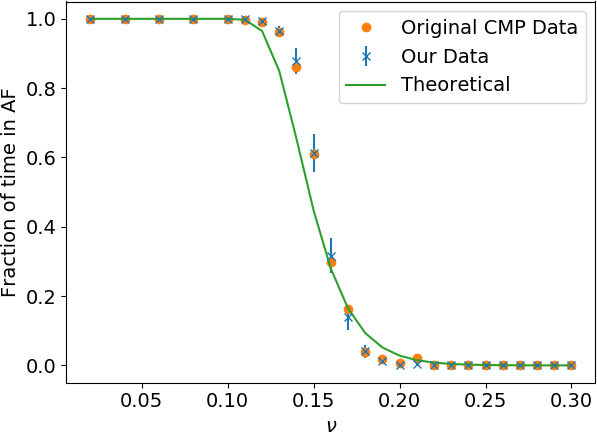
\includegraphics[width=0.66\textwidth]{cmp_risk_curve}
    \caption[short caption]{The CMP `risk curve', so-called because it shows how the risk of AF varies with $\nu$. When generating our data, 50 different lattices were generated at each point in a graph, and the fraction of time fibrillating was measured over $10^6$ timesteps in each. Hence each point on the graph is a mean over 50 runs, and the error bars are calculated using the standard error of the mean. The data from our implementation shows good agreement with the data from the original implementation by \etalcite{cmp}{Christensen}. The agreement with theory is reasonable, but there is some departure due to boundary effects, as these are neglected when deriving the theoretical form~\cite{manani}. 
    At small $\nu$, the atria are in persistent fibrillation. At high $\nu$ there is no fibrillation. There is a `transition region' in the middle where the heart spends a finite amount of time fibrillating, which we describe as `paroxysmal'. }
\label{fig:cmpriskcurve}
\end{mdframed} \end{figure}

\clearpage
\section{Methodology from Our CMP Implementation}

We implemented the CMP model from scratch to develop a proof-of-concept algorithm to find re-entry circuits, that we later generalised to a more realistic topology.

\subsection{Verification}

First, we verified that the model had been correctly implemented by reproducing the risk curve from the original CMP paper. In order to do this, we randomly generated $50$ lattices for each value of $\nu$ under consideration. Then, the model was run for $10^6$ timesteps for each lattice. The fraction of time spent fibrillating was recorded for each lattice, and mean fraction was plotted against $\nu$ in Fig.~\ref{fig:cmpriskcurve}. Our data showed good agreement with the risk curve data from the original CMP paper, confirming that the implementation of the algorithm was valid. There was some error in the measured fraction due to the time at the start of the simulation when the model had not yet had time to start fibrillating. This was mitigated by running for a number of timesteps that is much larger than the pacemaker period ($10^6 \gg T$).

\subsection{Locating Re-entry Circuits} \label{sec:locating}

We developed an algorithm that will eventually find the shortest re-entry circuit currently active in the model. We first ran the model until fibrillation arose. The algorithm, explained in Fig.~\ref{fig:reentryalgo}, builds a tree structure to locate looping signals. We defined it in a general way that doesn't depend on the structure of the CMP lattice, so it becomes easy to generalise to higher dimensions or more complicated geometries. It is intentionally iterative rather than recursive, which reduces the number of slow Python function calls.

\begin{figure} \begin{mdframed}
    \centering
    \begin{subfigure}[b]{0.46\textwidth}
        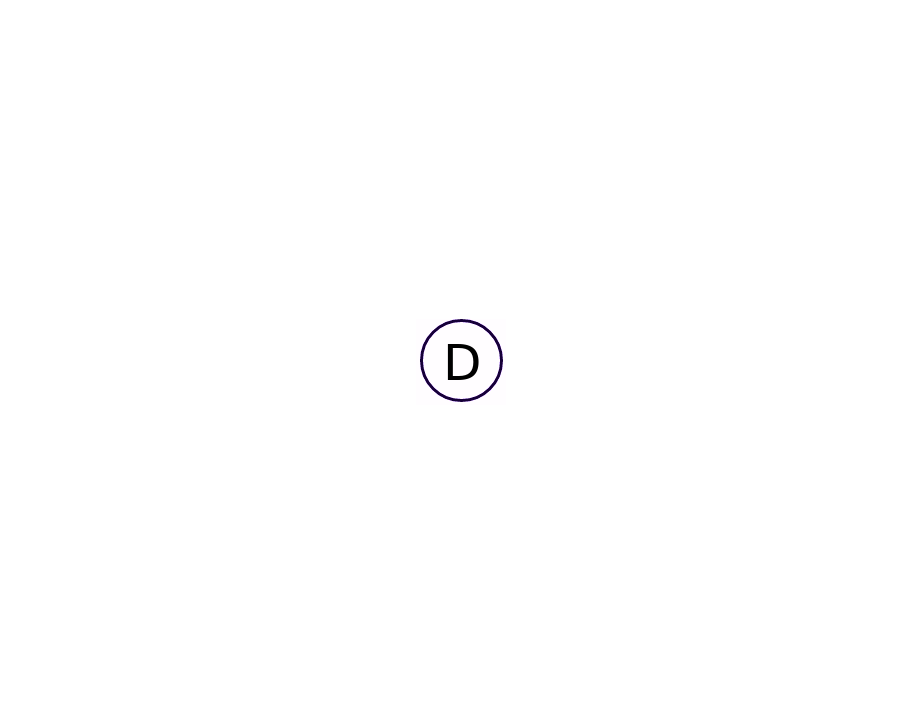
\includegraphics[width=\textwidth, trim={0cm 6cm 0 6cm}, clip]{tree_1}
        \caption{The algorithm starts by creating a tree with a single node (referred to as the `root node'), representing the cell that was first excited more times than the pacemakers. We define $t$ to be the time at which it becomes excited more times than the pacemakers. Therefore, at $t$ the re-entry circuit has just completed its first loop. Any node corresponding to this cell is labelled D. \\}
    \end{subfigure}
    ~
    \begin{subfigure}[b]{0.46\textwidth}
        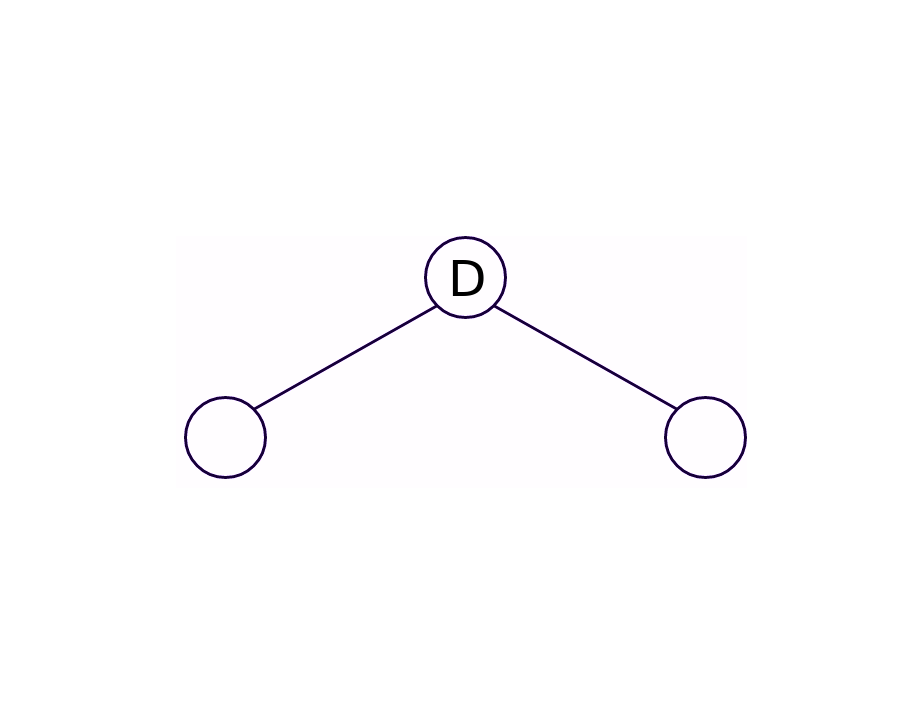
\includegraphics[width=\textwidth, trim={0 6cm 0 6cm}, clip]{tree_2}
        \caption{Cells that are coupled to the start cell and are excited at time $t-1$ are added as children to the root node. In this exemplar case there are two such cells. The next step in the algorithm will be to consider the excited neighbours of these two cells at time $t - 2$, adding them as grandchildren to the root node. \\ \\}
    \end{subfigure}
    
    \begin{subfigure}[b]{0.92\textwidth}
        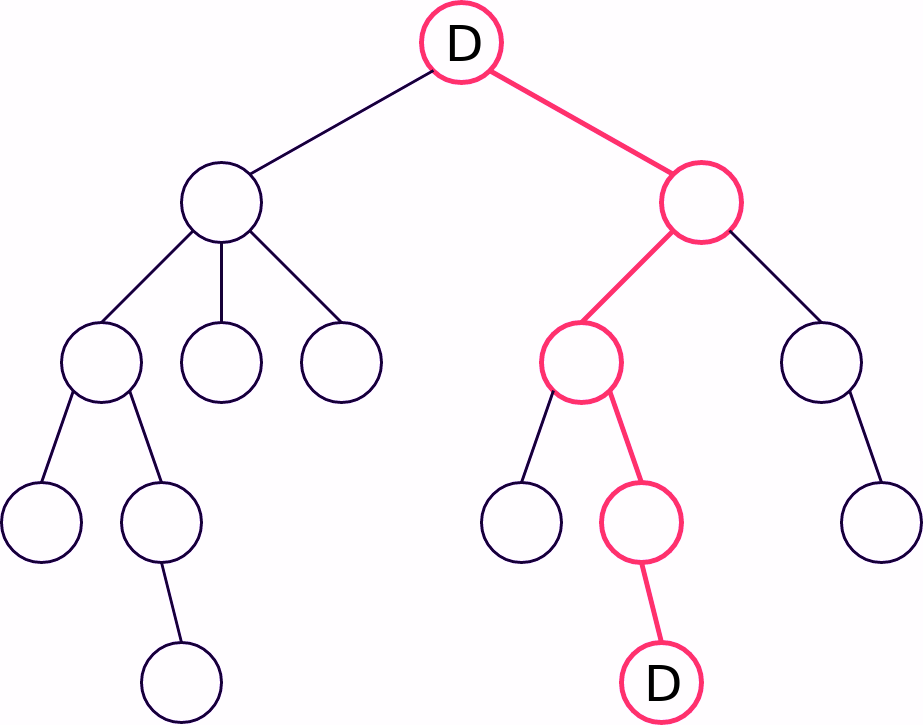
\includegraphics[width=\textwidth]{tree_3}
        \caption{This process is repeated until the original cell cell is added to the tree again. Once this happens we can trace a route (red) from the original cell at the bottom to the root node. The nodes lying on this route represent the cells in the circuit.}
    \end{subfigure}
    % \end{mdframed}
    \caption{Our algorithm used to locate re-entry circuits. It always finds the shortest re-entry circuit active in the model. It must be stressed that this is a highly simplified example; our real trees are much larger and more complicated.}
    \label{fig:reentryalgo}
\end{mdframed} \end{figure}

\subsection{Centrality Measurements} \label{sec:centrality}

The circuit-finding algorithm defined in Sec.~\ref{sec:locating} is computationally intensive, so a more computationally efficient proxy for re-entrant activity is desirable.
As previously established, for a re-entry circuit to form, transverse connections must be sufficiently far apart. This requires a fibre to be mostly isolated, which necessarily means cells on that fibre will have few connections. 

Centrality measures quantify how well-connected a particular site is, which means that cells on an isolated fibre would have low centrality. Many of these are extremely computationally intensive for large numbers of sites, or consider scales much greater than the size of a re-entry circuit.
However, a less computationally intensive option is harmonic centrality:
\begin{equation}
    H_i = \sum_{j \ne i}^N \frac{1}{d_{ij}}, \label{eq:harmonic}
\end{equation}
where $i$ is the index of the cell for which we want to calculate centrality, $N=40,000$ is the number of cells, and $d_{ij}$ is the minimum number of connections that have to be traversed in order to reach cell $i$ from cell $j$. We expected this to be useful because unlike many other centrality measurements, it weights the local area around cell $i$ very highly. One can see that cells on an isolated stretch of fibre are going to have a much lower value of $H_i$ than those on a well-connected stretch, as the shortest path to most other sites will have to go through a long stretch of isolated fibre. Thus we would expect low centrality to indicate high re-entrant activity.

The time required to calculate $H_i$ for $N$ sites would scale as $\sim N^2$. However, since the CMP model is homogeneous on large scales, one does not need to actually sum all the way up to $N$ to calculate $H_i$; instead one can sum over all sites with $d_{ij} < D$, where $D$ is some threshold distance greater than the length of a typical isolated stretch. The terms that are neglected average out to a `background' contribution that is approximately the same at any point in the lattice. This turns a problem that is quadratic in $N$ into a problem with more favourable complexity. Preliminary tests found that there was no noticeable difference between $D=20$ and $D\rightarrow\infty$, so we chose $D=20$ as our cutoff.

\section{Results from Our CMP Implementation}

For illustrative purposes, a plot showing re-entry circuits next to reciprocal centrality measurements (i.e. $1 / H_i$) is shown in Fig.~\ref{fig:centralitycomparison}; there appears to be some correlation but it is difficult to ascertain how strong this correlation is. Figure~\ref{fig:cvcall} shows how well centrality predicts re-entrant activity. We found that low centrality is a good predictor of re-entrant activity, and that low centrality is a much better predictor at values of $\nu$ within the transition region than outside. Low centrality is a worse predictor at very small $\nu$ because re-entry circuits can form almost anywhere and centrality is low almost everywhere.

\begin{figure}[h!] \begin{mdframed}
    \centering
    \begin{subfigure}[b]{0.46\textwidth}
        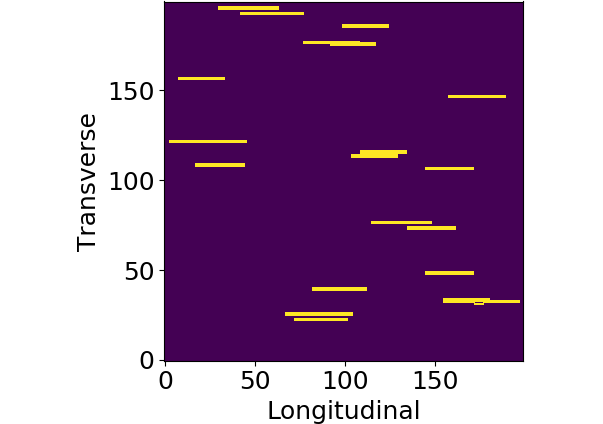
\includegraphics[width=\textwidth]{circuit_map_binary}
        \caption{The locations of the re-entry circuits found for a particular lattice. Most of the circuits are long and narrow like the example in Fig.~\ref{fig:cmpreentry}, so in this visualisation (in which there are no gaps between adjacent cells) they look like bars.}
    \end{subfigure}
    ~
    \begin{subfigure}[b]{0.46\textwidth}
        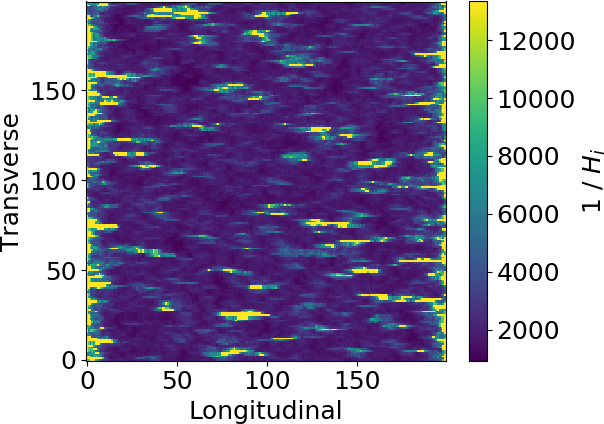
\includegraphics[width=\textwidth]{centrality_harmonic_reciprocal}
        \caption{The centrality measurements for the cells on the lattice. We have shown the reciprocal because low centrality is associated with re-entry circuits. The centrality is lower at the left and right edges because those cells have fewer neighbours.}
    \end{subfigure}
    \caption{Side by side comparison of re-entrant activity and centrality measurements for a particular lattice with $\nu = 0.14$. Ignoring the edge-effects in (b), there is correlation. Axis units are integer grid coordinates rather than real distance measurements.}
\label{fig:centralitycomparison}
\end{mdframed} \end{figure}

\begin{figure}
    \begin{mdframed}
    \centering
    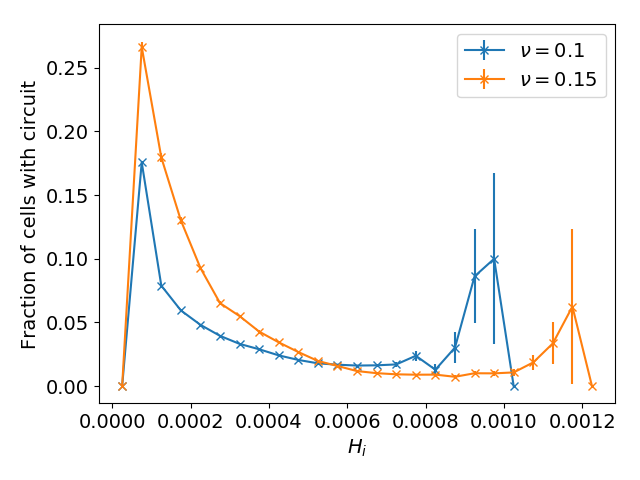
\includegraphics{circuits_v_centrality_harmonic_ALL}
    \caption{How well does centrality predict re-entry? Inside the transition region at $\nu=0.15$, a cell with very low centrality has a 26\% chance of hosting a re-entry circuit, but outside the transition region centrality is a worse predictor. The spike at high centrality is likely because high-centrality cells have many pathways going through them, so re-entry circuits happen to pass through them as a matter of chance. Though the data is binomial (as each cell either has a circuit or not), there are many points in each bin so a Gaussian approximation was used to calculate the standard error of the mean for the error bars.}
    \label{fig:cvcall}
\end{mdframed} \end{figure}

\clearpage
\section{Implementation} \label{sec:cmpimpl}

We implemented the CMP model ourselves in C++, providing a Python interface through the Python/C~API. This has all the performance advantages of C++, while allowing NumPy for data analysis and Matplotlib for producing high-quality visualisations. This fast, flexible implementation would not be feasible using either language in isolation.

We implemented from scratch all the code required to run this model, find re-entry circuits, and measure centrality. This required 1722 lines of Python code and 1512 lines of C++ code, with 81 lines in miscellaneous build scripts. The total number of lines of code was 3315. We used no external libraries other than the standard Python libraries, Matplotlib, and NumPy.

We used several techniques to improve performance, besides improvements to algorithmic complexity already mentioned. Finely tuning the compiler with the aid of profiling tools allowed for powerful optimisations in performance critical areas of the code; with this information we found seemingly trivial changes like reversing loop orders and replacing modulo operations with if-statements saw speed increases of around 10\% each. When calculating statistics we leveraged multiprocessing in order to spread the workload across several CPU cores at once. Instead of applying the algorithm described in Fig.~\ref{fig:cmpalgo} to every cell, we kept track of excited cells and only considered the cells bordering them; this produced identical behaviour whilst having to loop over fewer cells. We used bitmasks (binary numbers where the individual bits represent booleans such as presence of connections or whether a cell is defective) to store properties of each cell as this gave significant performance gains and saved on memory. We avoided using nested structures such as vectors of vectors, preferring to flatten these lists to make use of CPU caching.

\section{Key Points from Chapter \thechapter}

\begin{itemize}
    \item The CMP model is a cellular automaton that obeys simple rules, summarised in Fig.~\ref{fig:cmpalgo}. These rules are based on the behaviour of real heart cells.
    \item We define the model to be fibrillating when any non-pacemaker cell has been excited more times than the pacemakers.
    \item The CMP model has a control parameter $\nu$ which is analogous to fibrosis in the real heart, and affects risk of AF.
    \item We have designed an algorithm to find re-entry circuits that is easily generalised to higher dimensions and more complex geometries.
    \item Low harmonic centrality is a good predictor of re-entrant activity.
\end{itemize}
